\chapter{Kort}
\label{kort}

\begin{center}
\begin{figure}[H]
\begin{center}
\subfigure{
\includegraphics[scale=0.8]{images/implementation/kort-icon_with_gloss}}
\hspace{1cm}
\subfigure{
\includegraphics[scale=0.8]{images/implementation/kort_herokuapp_com-qrcode}}
\end{center}
\end{figure}

{\large \textbf{\url{http://kort.herokuapp.com/}}}

\vspace{1cm}

\begin{figure}[H]
\subfigure{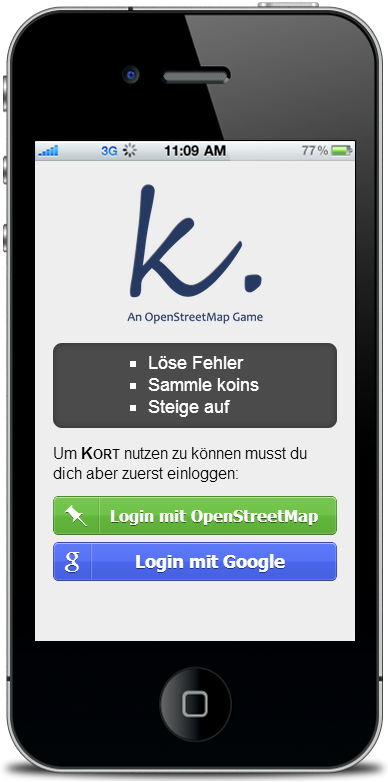
\includegraphics[width=0.3\textwidth]{images/screenshots/kort-screenshot-login}}
\hfill
\subfigure{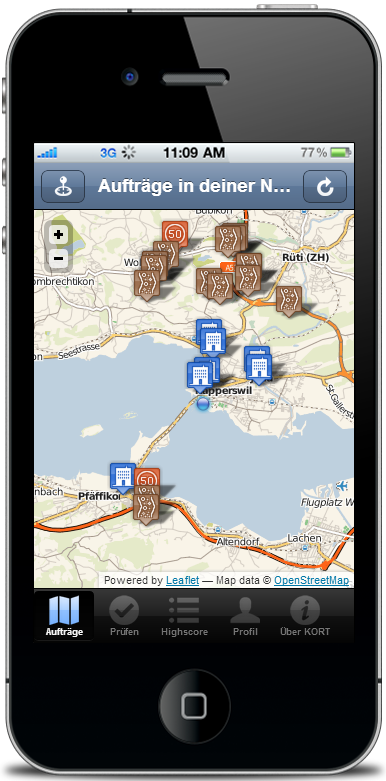
\includegraphics[width=0.3\textwidth]{images/screenshots/kort-screenshot-bugmap}}
\hfill
\subfigure{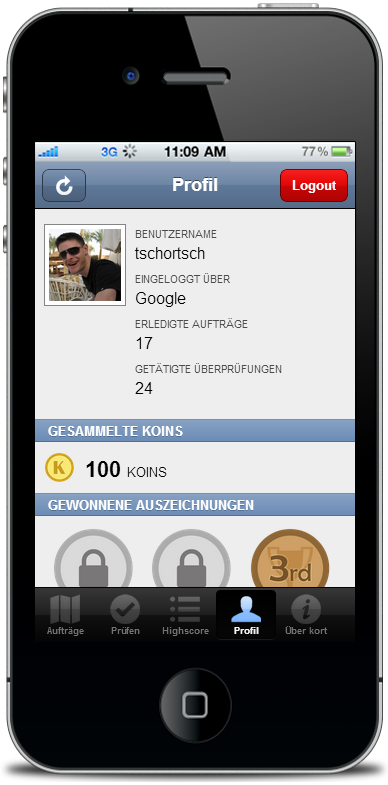
\includegraphics[width=0.3\textwidth]{images/screenshots/kort-screenshot-profile}}
\end{figure}
\end{center}

% Einführung
\section{Einführung}
\subsection{Idee}


% Ziel
\subsection{Ziel}


% Analyse
\section{Analyse}

% Subfigure counter zuruecksetzen
\setcounter{subfigure}{0}

\subsection{Paper-Prototype}
Vor der Implementation der Oberfläche wurde ein Paper-Prototype des GUI-Designs erstellt.
Der Prototype besteht aus vier Hauptmasken und einem Overlay für den Login.

\subsubsection{Overlay: Login}
Beim ersten Starten der \gls{WebApp} erhält man die Möglichkeit sich über verschiedene Dienste anzumelden.
Beim Klick auf den jeweiligen Anbieter wird man zu diesem Weitergeleitet und kann sich dort anmelden.

\begin{figure}[H]
\subfigure[Login - Anbieterauswahl]{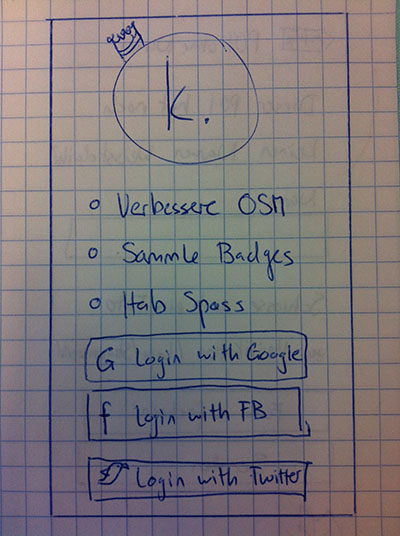
\includegraphics[width=0.43\textwidth]{images/paperprototype/kort-pp-startscreen}}
\hfill
\subfigure[Login - Loginformular des jeweiligen Anbieters]{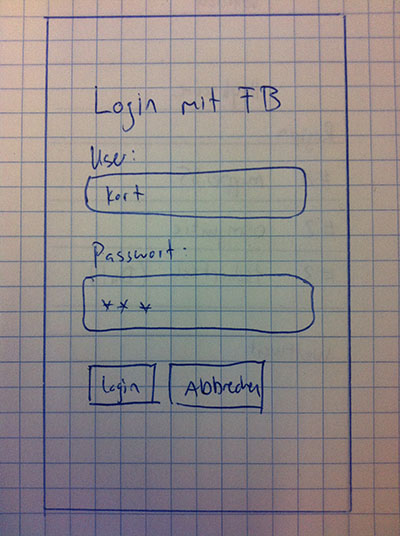
\includegraphics[width=0.43\textwidth]{images/paperprototype/kort-pp-login}}
\end{figure}

\subsubsection{Maske: Aufträge}
Ist der Login erfolgt erscheint die Maske mit den Aufträgen.
Darauf ist werden die bestehenden Fehler auf einer Karte angezeigt.
Es werden jeweils nur die Fehler angezeigt, welche sich in unmittelbarer Nähe vom eigenen Standort befinden.
Die Fehler werden mit einer Markierung auf der Karte dargestellt.

Durch Anklicken einer solchen Markierung öffnet sich die Detailansicht des Fehlers, worin sich der Fehler direkt beheben lässt.
Neben der Möglichkeit einen Lösungstext einzugeben, soll es auch möglich sein ein Beweis-Foto dazu hochzuladen.
Mit einem Klick auf Senden schliesst sich die Detailansicht und man sieht wieder die Karte.

\begin{figure}[H]
\subfigure[Aufträge - Karte mit Fehlern]{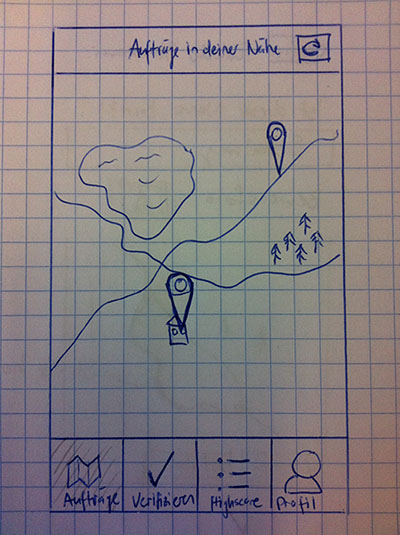
\includegraphics[width=0.43\textwidth]{images/paperprototype/kort-pp-bugs}}
\hfill
\subfigure[Aufträge - Detailansicht eines Fehlers]{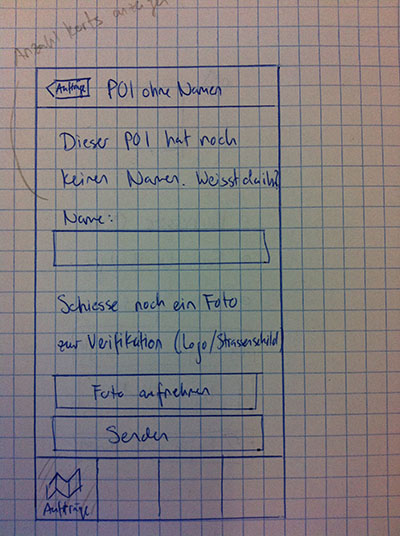
\includegraphics[width=0.43\textwidth]{images/paperprototype/kort-pp-fix}}
\end{figure}

\subsubsection{Maske: Verifizieren}
Auf der Verifikationsmaske werden die bereits gelösten Fehler in der Nähe angezeigt.
Sie sind gruppiert nach Anzahl nötigen Verifikationen, um sie zu OpenStreetMap zurückzusenden.

Per Klick auf einen Eintrag öffnet sich die Verifikationsmaske.
Darin wird der Fehlerlösungstext und das Beweis-Foto angezeigt.
Zusätzlich wird das betroffene OpenStreetMap-Objekt auf einer Karte angezeigt.
Man hat die Möglichkeit die Problemlösung als \emph{Korrekt} oder \emph{Falsch} zu werten.

\begin{figure}[H]
\subfigure[Verifizieren - Liste mit Fehlerlösungen]{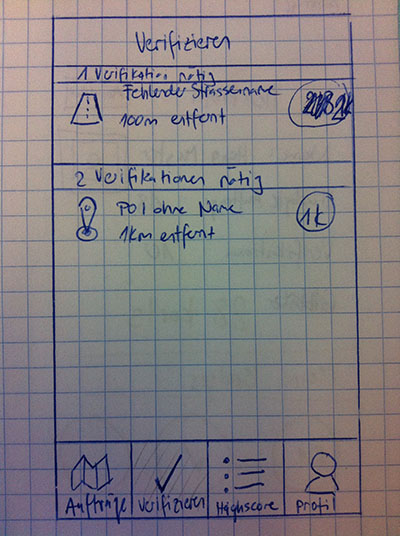
\includegraphics[width=0.43\textwidth]{images/paperprototype/kort-pp-verify}}
\hfill
\subfigure[Verifizieren - Detailansicht einer Fehlerlösung]{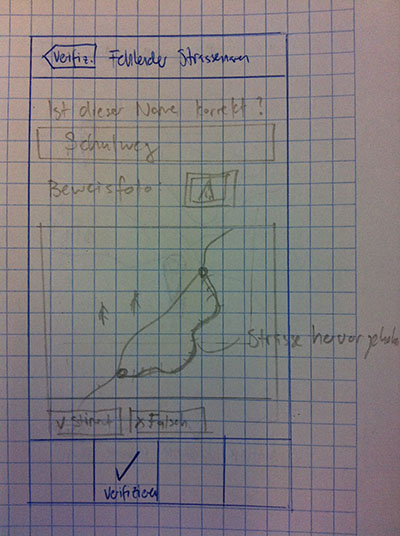
\includegraphics[width=0.43\textwidth]{images/paperprototype/kort-pp-verify_detail}}
\end{figure}

\subsubsection{Masken: Highscore / Profil}
In der Highscore-Maske hat man die Möglichkeit sich mit anderen Spielern vergleichen.
Man sieht seine eigene und die Platzierungen der anderen Spieler.
Es werden Highscores für verschiedene Kategorien (z.B. Regional, Weltweit) angezeigt.

Im Profil sieht man einen Steckbrief seines eigenen Benutzers.
Es wird angezeigt wieviele Aufträge man gelöst und wieviele Verifikationen man getätigt hat.
Zusätzlich werden die Gesamtanzahl der gesammelten Punkte und die gewonnenen Badges angezeigt.
Die Profil-Maske bietet zudem die Möglichkeit sich von der App abzumelden.

\begin{figure}[H]
\subfigure[Highscore]{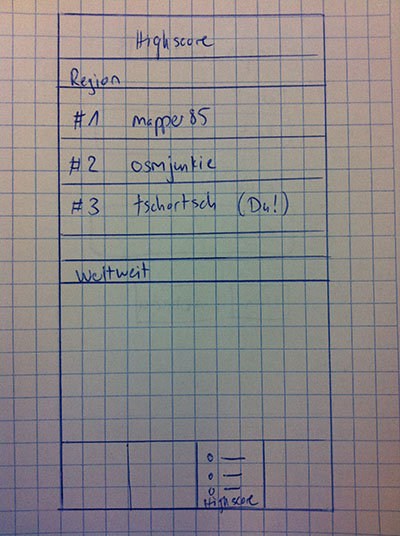
\includegraphics[width=0.43\textwidth]{images/paperprototype/kort-pp-highscore}}
\hfill
\subfigure[Profil]{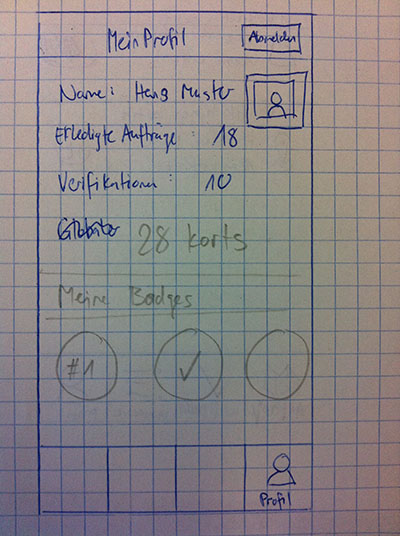
\includegraphics[width=0.43\textwidth]{images/paperprototype/kort-pp-profile}}
\end{figure}

% Design
\section{Design}

% Implementation
\section{Implementation}

\subsection{Starten der App}
Beim Starten der App wird duch mehrere Entscheidungen festgelegt, welche Maske dem Benutzer angezeigt wird. In Abbildung \ref{image-kort-startup-activitydiagram} ist der Ablauf grob dargestellt.

\begin{figure}[H]
	\centering
	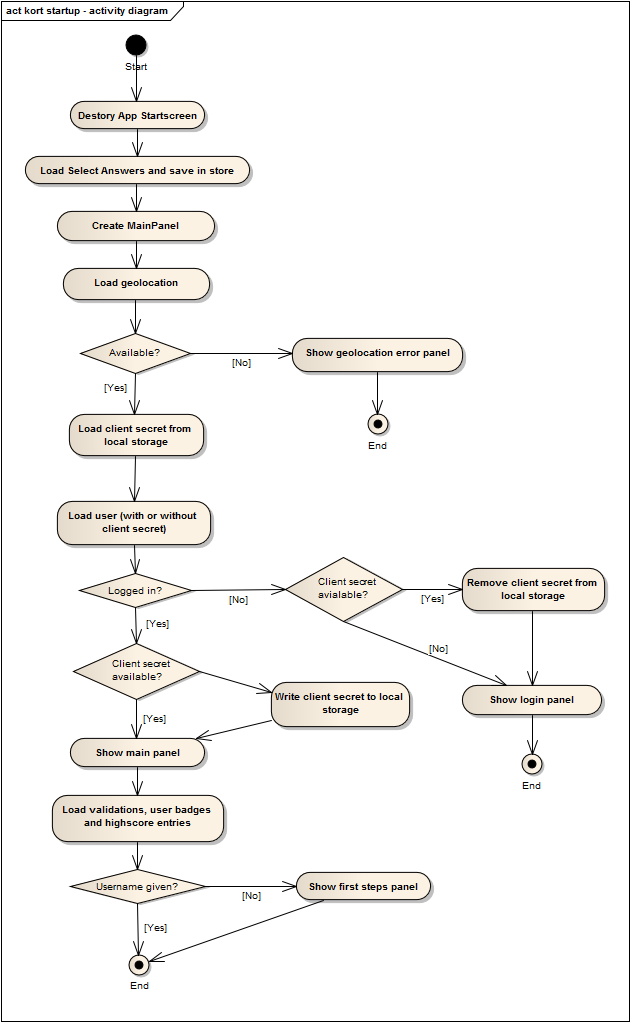
\includegraphics[scale=0.55]{images/uml/kort-startup-activitydiagram}
	\caption{Ablauf beim Starten der App}
	\label{image-kort-startup-activitydiagram}
\end{figure}

Schlussendlich wird dem Benutzer eine der folgenden Masken angezeigt:

\begin{itemize}
\item Geolocation Fehler Maske: Wenn Geolocation nicht gelesen werden kann.
\item Login Maske: Wenn Benutzer noch nicht eingeloggt ist
\item Erste Schritte Maske: Wenn Benutzer noch keinen Benutzernamen gewählt hat
\item Hauptmaske: Falls alles andere geklappt hat
\end{itemize}

\subsection{Sencha Cmd}
\label{sencha-cmd}
Das Grundgerüst der App wurde komplett mit dem Sencha-eigenen Build-Tool \emph{Sencha Cmd 3.0.0}\footnote{\url{http://www.sencha.com/products/sencha-cmd}} generiert.
Dieses bietet verschiedene Build-Möglichkeiten an:

\begin{table}[H]
\centering
\begin{tabular}{|p{0.2\twocelltabwidth}|p{0.8\twocelltabwidth}|}
\hline
\textbf{Build} & \textbf{Beschreibung} \\
\hline
testing & Bei diesem Build werden die JavaScript-Quelldateien in einer Datei zusammengefasst. Zusätzlich werden lediglich die verwendeten Dateien kopiert. \\
\hline
production & Der Production-Build entspricht grundsätzlich dem Testing-Build. Zusätzlich werden aber noch die JavaScript-Quelldateien komprimiert. \\
\hline
package/native & Mit diesen Builds lassen sich native Apps für die verschiedenen mobilen Betriebssysteme generieren. \\
\hline
\end{tabular}
\caption{Verschiedene Build-Möglichkeiten mit Sencha Cmd}
\label{table-sencha-cmd-build}
\end{table}

Durch den Einsatz von Sencha Cmd wird es möglich mit einem geringen Mehraufwand, eine native App zu generieren und diese in den verschiedenen App-Stores (Apples AppStore, Google Play Store) anzubieten.

\subsubsection{Konfiguration}
Der Buildprozess wird in der Datei \inlinecode{app.json} konfiguriert.

\begin{table}[H]
\centering
\begin{tabular}{|p{0.2\twocelltabwidth}|p{0.8\twocelltabwidth}|}
\hline
\textbf{Property} & \textbf{Beschreibung} \\
\hline
\inlinecode{"js"} & Hier können die JavaScript-Quelldateien, welche von der App verwendet werden eingetragen werden. Diese werden im Buildprozess automatisch in den \inlinecode{<head>}-Bereich des \inlinecode{index.html}-Files geschrieben. \\
\hline
\inlinecode{"css"} & Ähnlich wie das \inlinecode{"js"}-Property nur für CSS-Ressourcen. \\
\hline
\inlinecode{"ressources"} & Hier können weitere Ressourcen wie Grafiken oder Libraries angegeben werden. \\
\hline
\end{tabular}
\caption{Wichtige Konfigurations-Eigenschaften in Sencha Cmd (app.json)}
\label{table-sencha-cmd-appjson}
\end{table}

Zusätzlich ist in der Datei \inlinecode{.sencha/app/sencha.cfg} der Classpath für die App definiert.

Weitere Informationen zur Konfiguration findet man im entsprechendem Guide der Sencha Docs\footnote{\url{http://docs.sencha.com/touch/2-1/\#!/guide/command\_app}}.

\subsection{Internernationalisierung (i18n)}
\label{i18n}
Die Oberfläche von \textsc{Kort} wurde bereits für eine mögliche Übersetzung vorbereitet.
Dazu wurde das Plugin \emph{Ext.i18n.Bundle-touch}\footnote{\url{https://github.com/elmasse/Ext.i18n.Bundle-touch}} für Sencha Touch eingesetzt. Dieses ermöglicht es einzelne Texte in externen Sprach-Property-Files auszulagern.

Bei \textsc{Kort} befinden sich diese Files im Verzeichnis \inlinecode{/resources/i18n/} und müssen nach folgendem Schema benannt werden: \inlinecode{Kort\_<locale>.props}.
Die verwendete Sprache ist in der Funktion \inlinecode{prepareI18n()} der Datei \inlinecode{app.js} festgelegt.

\lstset{language=JavaScript}
\begin{lstlisting}[caption=kort - Sprache definieren, label=kort-choose-language]
prepareI18n: function() {
	Ext.i18n.Bundle.configure({
		bundle: 'Kort',
		language: 'de-CH',
		path: 'resources/i18n',
		noCache: true
	});
}
\end{lstlisting}

Hier kann über das \inlinecode{language}-Property die Sprache konfiguriert werden.
Falls das Property weggelassen wird, wird die aktuelle Spracheinstellung des Browsers verwendet.
Wird dabei die entsprechende Datei nicht gefunden, verwendet das Plugin die Datei \inlinecode{Kort.props}.

% Testing
\section{Testing}

% Resultate
\section{Resultate}

\subsection{Bekannte Fehler}

\subsubsection{iOS - Add to homescreen}
Eine sehr nützliche Funktionalität, welche Apple im Mobile Safari-Browser anbietet ist die \emph{Add to homescreen}-Funktion.

\begin{figure}[H]
\subfigure{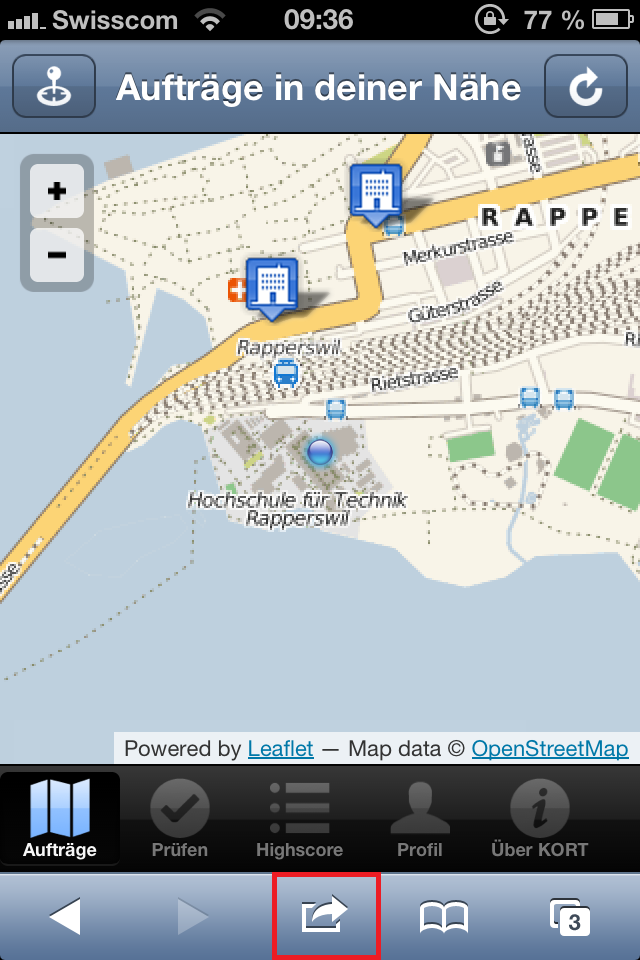
\includegraphics[width=0.23\textwidth]{images/bugs/kort-add_to_homescreen_1}}
\hfill
\subfigure{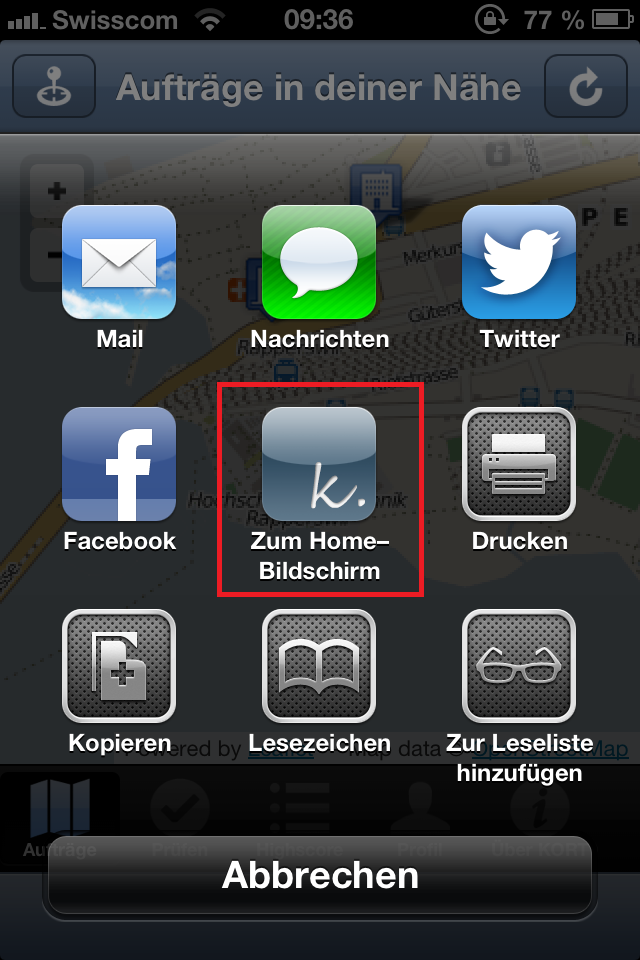
\includegraphics[width=0.23\textwidth]{images/bugs/kort-add_to_homescreen_2}}
\hfill
\subfigure{
\includegraphics[width=0.23\textwidth]{images/bugs/kort-add_to_homescreen_3}}
\hfill
\subfigure{
\includegraphics[width=0.23\textwidth]{images/bugs/kort-add_to_homescreen_4}}
\caption{iOS - "`Add to homescreen"'-Funktion}
\end{figure}

Dadurch wird ein App-ähnlicher Bookmark der aktuellen Webseite auf dem Homescreen erstellt.
Dieser erhält ein hinterlegtes Icon und einen Titel.
Beim Starten der App erscheint ein Splashscreen, welchen man ebenfalls in der Webseite definieren kann. Zudem öffnet sich der Browser ohne jegliche Toolbars wie der Adressleiste oder der Navigationsbar.

Leider hat die verwendete Version (2.1.0) des Sencha Touch Frameworks Fehler bei der Anzeige von einigen GUI-Komponenten.
So werden in unserem Fall die Karte (Aufträge) und alle Listen (Prüfen, Highscore) nicht korrekt dargestellt.

\subsubsection{App Build}
Wie in Abschnitt \ref{sencha-cmd} beschrieben, basiert die App vollständig auf dem Sencha-eigenen Build-Tool \emph{Sencha Cmd 3.0.0}. Darin sind aber noch einige Bugs vorhanden.

Bei \textsc{Kort} besteht dabei ein Problem bei der fest eingebauten Komprimierung der JavaScript-Sourcen.
Während diesem Prozess werden lokale Variablennamen mit einzelnen Buchstaben abgekürzt.
Dabei treten Konflikte mit der Leaflet-Library auf, welche den Buchstaben \emph{L} als Namespace verwendet. 